\documentclass[paper=letter, fontsize=11pt]{scrartcl} 
 \usepackage[top=2.5cm, bottom=2.5cm, left=2.5cm, right=2.5cm]{geometry}
\usepackage{framed}

\usepackage{graphicx}
\usepackage{verbatim}
\usepackage{pictex}  
\usepackage{multimedia}
\usepackage{listings}
\usepackage{xcolor,colortbl}
\usepackage[spanish]{babel} % language/hyphenation
\usepackage{amsmath,amsfonts,amsthm} % Math packages
\usepackage{amsbsy}
\usepackage{amssymb}
\usepackage{fancyvrb}
\usepackage{sectsty} % Allows customizing section commands
\usepackage[dvipsnames]{xcolor}

\newcommand{\defi}[3]{\textbf{Definición:#3}}
\newcommand{\fin}{$\blacksquare.$}
\newcommand{\finf}{\blacksquare.}
\newtheorem{thm}{Teorema:}

\newcommand{\grstep}[2][\relax]{%
   \ensuremath{\mathrel{
       {\mathop{\longrightarrow}\limits^{#2\mathstrut}_{
                                     \begin{subarray}{l} #1 \end{subarray}}}}}}
\newcommand{\swap}{\leftrightarrow}

\newcommand{\gen}{\text{gen}}

\newtheorem{thmt}{Teorema:}
\newtheorem{thmd}{Definición:}
\newtheorem{thml}{Lema:}
\newtheorem{thmj}{Ejemplo:}

\allsectionsfont{\centering \normalfont\scshape} % Make all sections centered, the default font and small caps
\usepackage{float}
\usepackage{fancyhdr} % Custom headers and footers
\pagestyle{fancyplain} % Makes all pages in the document conform to the custom headers and footers
\fancyhead{} % No page header - if you want one, create it in the same way as the footers below
\fancyfoot[L]{} % Empty left footer
\fancyfoot[C]{} % Empty center footer
\fancyfoot[R]{\thepage} % Page numbering for right footer
\renewcommand{\headrulewidth}{0pt} % Remove header underlines
\renewcommand{\footrulewidth}{0pt} % Remove footer underlines
\setlength{\headheight}{13.6pt} % Customize the height of the header
\usepackage{biblatex}
\addbibresource{references.bib}
\numberwithin{equation}{section} % Number equations within sections (i.e. 1.1, 1.2, 2.1, 2.2 instead of 1, 2, 3, 4)
\numberwithin{figure}{section} % Number figures within sections (i.e. 1.1, 1.2, 2.1, 2.2 instead of 1, 2, 3, 4)
\numberwithin{table}{section} % Number tables within sections (i.e. 1.1, 1.2, 2.1, 2.2 instead of 1, 2, 3, 4)

\setlength\parindent{0pt} % Removes all indentation from paragraphs - comment this line for an assignment with lots of text

\newcommand{\horrule}[1]{\rule{\linewidth}{#1}} % Create horizontal rule command with 1 argument of height

\title{	
\normalfont \normalsize 
\textsc{Centro de Investigaci\'on en Matem\'aticas (CIMAT). Unidad Monterrey} 
\\ [25pt] 
\horrule{0.5pt} \\[0.4cm] % Thin top horizontal rule
\huge Tarea 2 \\ 
\horrule{2pt} \\[0.5cm] % Thick bottom horizontal rule
}


\author{Enrique Santibáñez Cortés} % Your name

\date{\normalsize\today} % Today's date or a custom date

\begin{document}
\lstdefinestyle{customc}{
  belowcaptionskip=1\baselineskip,
  basicstyle=\footnotesize, 
  frame=lrtb,
  breaklines=true,
  %frame=L,
  %xleftmargin=\parindent,
  language=C,
  showstringspaces=false,
  basicstyle=\footnotesize\ttfamily,
  keywordstyle=\bfseries\color{green!40!black},
  commentstyle=\itshape\color{red!40!black},
  identifierstyle=\color{blue},
  stringstyle=\color{purple},
}

\lstset{breakatwhitespace=true,
  basicstyle=\footnotesize, 
  commentstyle=\color{green},
  keywordstyle=\color{blue},
  stringstyle=\color{purple},
  language=C++,
  columns=fullflexible,
  keepspaces=true,
  breaklines=true,
  tabsize=3, 
  showstringspaces=false,
  extendedchars=true}

\lstset{ %
  language=R,    
  basicstyle=\footnotesize, 
  numbers=left,             
  numberstyle=\tiny\color{gray}, 
  stepnumber=1,              
  numbersep=5pt,             
  backgroundcolor=\color{white},
  showspaces=false,             
  showstringspaces=false,       
  showtabs=false,               
  frame=single,                 
  rulecolor=\color{black},      
  tabsize=2,                  
  captionpos=b,               
  breaklines=true,            
  breakatwhitespace=false,    
  title=\lstname,             
  keywordstyle=\color{blue},  
  commentstyle=\color{dkgreen},
  stringstyle=\color{mauve},   
  escapeinside={\%*}{*)},      
  morekeywords={*,...}         
} 


\maketitle

\section{Problema 1}
Considera una matriz de datos $X_{n\times d}$. PCA puede formularse también como el problema de encontrar un subespacio (ortonormal) de baja dimensión de forma tal que se minimicen los errores de las proyecciones de los datos en tal subespacio.\\
Si consideramos una base ortonormal $\{u_j\}, \ j = 1,\cdots , d$ , ya vimos que una observación $x_i$ puede expresarse como una combinación lineal $$\bf x_i =\sum_{j=1}^d \alpha_{ij} u_j.$$
Por la ortogonalidad de $\bf{u_j}$, podemos expresar $\alpha_{ij}=\bf x_i'u_j$. Entonces 
\begin{align}\label{xi}
\bf{x_i} = \sum_{j=1}^d (x_i'u_j)u_j.
\end{align}

Ahora, considera una aproximación basada en los primeros $p<d$ vectores de la base de acuerdo al modelo lineal: 
\begin{align}\label{xihat}
\bf \hat{x}_i=\sum_{j=1}^p z_{ij}u_j+\sum_{j=p+1}^d b_j u_j.
\end{align}

Observa que los coeficientes $z_{ij}$ \textit{dependen} de la observación $i$, mientras que $b_j$ son constantes para todas las observaciones.\\
Considera la minimización de la siguiente función de costo:
\begin{align}\label{funcion_costo}
L=\frac{1}{n} \sum_{i=1}^n \bf ||x_i-\hat{x}_i||^2.
\end{align}

\subsection{Encuentra los valores de $z_{ij}$, $b_j$ que minimizan la función de costo(\ref{funcion_costo})}
Tenemos que la base $\{u_j\}, \ j = 1,\cdots , d$ es ortonormal, es decir, se cumple que
\begin{itemize} \label{normal}
    \item $u_i \cdot u_j=0, \ \ \text{donde} \ i,j= 1,\cdots , d,| i\neq j.$
    \item $u_i \cdot u_i=1, \ \ \text{donde} \ i= 1,\cdots , d.$
\end{itemize}
Una vez aclarado la definición de base ortonormal, procedemos a encontrar los puntos de inflexión para $z_{ij}$ ocupando el criterio de primera derivada de la función de costo (\ref{funcion_costo}), pero primeros reescribiremos la función de costo ocupando (\ref{xi}) y (\ref{xihat}) de la siguiente manera:
\begin{align}\label{function_cost_new}
    L=\bf \frac{1}{n} \sum_{i=1}^n  ||x_i-\hat{x}_i||^2=\frac{1}{n} \sum_{i=1}^n \left| \left|\sum_{j=1}^d (x_i'u_j)u_j-\sum_{j=1}^p z_{ij}u_j-\sum_{j=p+1}^d b_j u_j. \right| \right|^2.
\end{align}
Entonces ocupando la primera derivada de la función de costo(\ref{function_cost_new}) con respecto a $z_{kl}$ donde $k\in \{1,2, \cdots,n\}, \ \ l\in \{1,2, \cdots, p\}$ es
\begin{align*}
    \bf \frac{\partial L}{\partial z_{kl}} = \frac{2}{n}\left( \sum_{j=1}^d (x_k'u_j)u_j-\sum_{j=1}^p z_{kj}u_j-\sum_{j=p+1}^d b_j u_j \right) \cdot \left(-u_l\right) 
\end{align*}
Ocupando (\ref{normal}) tenemos que $u_j \cdot u_l=0$ si $j\neq l$ y $u_j \cdot u_l=0$ si $j=l$, por lo que podemos simplificar la derivada como
\begin{align*}
    \bf \frac{\partial L}{\partial z_{kl}} &= \bf \frac{2}{n}\left( -\left(\sum_{j=1}^d (x_k'u_j)u_j\right)\cdot u_l+\left(\sum_{j=1}^p z_{kj}u_j\right)\cdot u_l+\left(\sum_{j=p+1}^d b_j u_j\right)\cdot u_l \right)\\
    & \bf = \frac{2}{n}\left( -\sum_{j=1}^d (x_k'u_j)u_j\cdot u_l+\sum_{j=1}^p z_{kj}u_j\cdot u_l+\sum_{j=p+1}^d b_j u_j\cdot u_l\right) \\
    & \bf = \frac{2}{n}\left( -\sum_{\substack{j=1 \\ j\neq l }}^d (x_k'u_j)u_j\cdot u_l+(x_k'u_l)u_l\cdot u_l+\sum_{\substack{j=1 \\ j\neq l }}^p z_{kj}u_j\cdot u_l+z_{kl}u_l\cdot u_l+\sum_{j=p+1}^d b_j u_j\cdot u_l\right) \\
    & \bf = \frac{2}{n}\left( -\sum_{\substack{j=1 \\ j\neq l }}^d (x_k'u_j)\cdot 0+(x_k'u_l)+\sum_{\substack{j=1 \\ j\neq l }}^p z_{kj}\cdot 0+z_{kl}+\sum_{j=p+1}^d b_j \cdot 0\right) \\
    &\bf =  \frac{2}{n}\left(-(x_k'u_l)+z_{kl}\right)
\end{align*}
Ocupando el criterio de primera derivada tenemos que el punto de inflexión es 
\begin{align*}
     \bf \frac{2}{n}\left(-(x_k'u_l)+z_{kl}\right)&=0\\
     \bf -(x_k'u_l)+z_{kl}&=0\\
     \bf z_{kl}&=\bf x_k'u_l.
\end{align*}
Ahora, la segunda derivada de la función de costo con respecto a $z_{kl}$ es 
\begin{align}
    \frac{\partial L}{\partial^2 z_{kl}} = \frac{2}{n}.
\end{align}
\textbf{Por lo tanto, como la segunda derivada es no negativa podemos concluir usando el criterio de segunda derivada que el punto  de inflexión $\bf z_{kl}&=\bf x_k'u_l$ es un mínimo.}\\

Realizando la misma metodología para encontrar el punto que minimiza la función de costo para $b_j$, tenemos que la primera derivada de la función de costo (\ref{function_cost_new}) con respecto a $b_h$ donde $h\in \{p+1,p+2, \cdots, d\}$ es  
\begin{align*}
    \bf \frac{\partial L}{\partial b_{h}} = \frac{2}{n}\sum_{i=1}^n \left( \sum_{j=1}^d (x_i'u_j)u_j-\sum_{j=1}^p z_{ij}u_j-\sum_{j=p+1}^d b_j u_j \right) \cdot \left(-u_h\right) 
\end{align*}
Ocupando (\ref{normal}) tenemos que $u_j \cdot u_h=0$ si $j\neq h$ y $u_j \cdot u_h=0$ si $j=h$, por lo que podemos simplificar la derivada como
\begin{align*}
    \bf \frac{\partial L}{\partial b_{h}} &= \bf  \frac{2}{n}\sum_{i=1}^n\left( -\left(\sum_{j=1}^d (x_i'u_j)u_j\right)\cdot u_h+\left(\sum_{j=1}^p z_{ij}u_j\right)\cdot u_h+\left(\sum_{j=p+1}^d b_j u_j\right)\cdot u_h \right)\\
    &\bf = \frac{2}{n}\sum_{i=1}^n\left( -\sum_{j=1}^d (x_i'u_j)u_j\cdot u_h+\sum_{j=1}^p z_{ij}u_j\cdot u_h+\sum_{j=p+1}^d b_j u_j\cdot u_h\right) \\
    &\bf = \frac{2}{n}\sum_{i=1}^n\left( -\sum_{\substack{j=1 \\ j\neq h }}^d (x_i'u_j)u_j\cdot u_h-(x_i'u_h)u_h\cdot u_h+\sum_{j=1}^p z_{ij}u_j\cdot u_h+\sum_{\substack{j=1 \\ j\neq h }}^d b_j u_j\cdot u_h+b_j u_h\cdot u_h\right) \\
    &\bf = \frac{2}{n}\sum_{i=1}^n\left(-\sum_{\substack{j=1 \\ j\neq h }}^d (x_i'u_j)\cdot 0-(x_i'u_h)+\sum_{j=1}^p z_{ij}\cdot 0+\sum_{\substack{j=1 \\ j\neq h }}^d b_j \cdot 0-b_j\right) \\
    &\bf =  \frac{2}{n}\sum_{i=1}^n\left(-x_i'u_h+b_{h}\right) =-\frac{2}{n}\sum_{i=1}^n x_i'u_h+2b_h=-2\bar{x}'u_h+2b_h.
\end{align*}
Ocupando el criterio de primera derivada tenemos que el punto de inflexión es 
\begin{align*}
     \bf -2\bar{x}'u_h+2b_h&=0\\
     \bf 2b_h&=\bf 2\bar{x}'u_h\\
     \bf b_h&=\bf \bar{x}'u_h.
\end{align*}
Ahora, la segunda derivada de la función de costo con respecto a $b_{h}$ es 
\begin{align*}
    \bf \frac{\partial L}{\partial^2 b_{h}} = 2.
\end{align*}
\textbf{Por lo tanto, como la segunda derivada es no negativa podemos concluir usando el criterio de segunda derivada que el punto  de inflexión $\bf b_{h}=\bar{x}'u_h$ es un mínimo.}\\

Ocupando los dos resultados anteriores, es decir, $z_{ij}=x_i'uj$ y $b_{j}=\bar{x}'u_j$ minimizan la función de costo tenemos que 
\begin{align*}
    \bf x_i-\hat{x}_i&= \bf \sum_{j=1}^d (x_i'u_j)u_j-\sum_{j=1}^p z_{ij}u_j-\sum_{j=p+1}^d b_j u_j\\
    &\bf =\sum_{j=1}^d (x_i'u_j)u_j-\sum_{j=1}^p (x_i'uj)u_j-\sum_{j=p+1}^d(\bar{x}'u_j) u_j\\
    &\bf =\sum_{j=1}^p (x_i'u_j)u_j+\sum_{j=p+1}^d (x_i'u_j)u_j-\sum_{j=1}^p (x_i'uj)u_j-\sum_{j=p+1}^d(\bar{x}'u_j) u_j\\
    &\bf = \sum_{j=p+1}^d (x_i'u_j)u_j-\sum_{j=p+1}^d(\bar{x}'u_j)u_j u_j=\sum_{j=p+1}^d (x_i'u_j)u_j-(\bar{x}'u_j)u_j\\
    &\bf =\sum_{j=p+1}^d (x_i'u_j-\bar{x}'u_j)u_j=\sum_{j=p+1}^d ([x_i'-\bar{x}']u_j)u_j=\sum_{j=p+1}^d ([x_i-\bar{x}]'u_j)u_j.
\end{align*}
Es decir, la “desviación” está en el espacio ortogonal de los componentes principales.

Por último, ocupando el resultado anterior podemos reescribir la función de costo original (\ref{funcion_costo}) como
\begin{align*}
    L&=\frac{1}{n} \sum_{i=1}^n \bf ||x_i-\hat{x}_i||^2\\
    &=\bf \frac{1}{n} \sum_{i=1}^n \bf \left|\left| \sum_{j=p+1}^d ([x_i-\bar{x}]'u_j)u_j\right|\right|^2\\
    &= \bf \frac{1}{n} \sum_{i=1}^n \bf \sqrt{\sum_{j=p+1}^d ([x_i-\bar{x}]'u_j)u_j \cdot \sum_{j=p+1}^d u_j^T(u_j^T[x_i-\bar{x}])}^2\\
    &= \bf \frac{1}{n} \sum_{i=1}^n \bf \left( \sum_{j=p+1}^d ([x_i-\bar{x}]'u_j)u_j \cdot \sum_{j=p+1}^d u_j^T(u_j^T[x_i-\bar{x}])\right)\\
    &= \bf \frac{1}{n} \sum_{i=1}^n\left( \sum_{j=p+1}^d \left(\ [x_i-\bar{x}]'u_j\right)^2+\sum_{j=p+1}^d\sum_{\substack{\bf k=p+1\\ \bf k\neq j}}^p ([x_i-\bar{x}]'u_j)\underbrace{\bf u_j u_k^T}_{=0}(u_k^T[x_i-\bar{x}])\right)\\
    &= \bf \frac{1}{n} \sum_{i=1}^n\left( \sum_{j=p+1}^d \left(\ [x_i-\bar{x}]'u_j\right)^2\right) = \bf \frac{1}{n} \sum_{i=1}^n \sum_{j=p+1}^d  u_j^T[x_i-\bar{x}][x_i-\bar{x}]'u_j\\
    &= \bf \sum_{j=p+1}^d  u_j^T\left(\frac{1}{n} \sum_{i=1}^n[x_i-\bar{x}][x_i-\bar{x}]'\right)u_j = \bf \sum_{j=p+1}^d  u_j^TSu_j \ \ \blacksquare
\end{align*}
Es decir, la solución se puede obtener resolviendo un problema de valores propios. Esta propiedad ayuda a entender desde otro enfoque la metodología de PCA relacionándolo con la matriz de covarianzas. 

\section{Índice de Marginación en Nuevo León.}
\subsection{Introducción.}
La marginación se refiere como el conjunto de problemas (desventajas) sociales de una comunidad o localidad y hace referencia a grupos de personas y familias. Parte importante de estudiar la marginación nace de poder encontrar lugares en los que la marginación es más alta para poder ayudar con practicas reguladoras para cada estado, es decir, la marginación es un problema para la economía de los lugares, entonces a menores índices de marginación se esperaría una economía más alta o estable. \\

\subsection{Metodología}
Considerando que la marginación es importante, entonces hay que determinar como medirla. El Consejo Nacional de Población (CONAPO) ha presentado una metodología para medir la marginación a nivel localidad. La marginación se puede reflejar en tu nivel educativo, el lugar en que vives y el ingreso que percibes, por lo que para poder medirla hay que considerar estos tres aspectos: \textbf{educación, vivienda e ingreso económico}.\\

Con la ayuda del Censo 2010 que realizó el Instituto Nacional de Estadística, Geografía e Informática es posible medir estos tres aspectos para poder posteriormente tener una única medida de marginación.

Para medir la \textcolor{blue}{educación} consideramos dos indicadores, el primero se relaciona con la capacidad de las personas de leer y escribir un recado (analfabetas) y el segundo indicador se refiere a las personas que cursaron la primaria. Para la \textcolor{green}{vivienda} propuso 5 indicadores,  los cuales exploran las condiciones de las viviendas: carencia de excusado, carencia de servicio de energía eléctrica, uso de agua entubada, número de cuartos por personas en la vivienda y uso de piso de tierra. Y para el \textcolor{orange}{ingreso económico} un indicador, debido a que los datos del censo no presentan a un nivel localidad los ingresos económicos (por motivos de privacidad) se buscó un \textit{proxy}. La disponibilidad de refrigerador se encuentra condicionada por el ingreso del que se dispone en las viviendas, ya sea por trabajo o transferencias monetarias o en especie. \\

En resumen, los 8 indicadores a considerarla para medir la marginación a nivel localidad son:
\begin{enumerate}
    \item \textcolor{blue}{Porcentaje de población de 15 años o más analfabeta.}
    \item \textcolor{blue}{Porcentaje de población de 15 años o más sin primaria completa.}
    \item \textcolor{green}{Porcentaje de ocupantes en viviendas particulares habitadas sin drenaje ni excusado.}
    \item \textcolor{green}{Porcentaje de ocupantes en viviendas habitadas particulares habitadas sin energía eléctrica.}
    \item \textcolor{green}{Porcentaje de ocupantes en viviendas particulares habitadas sin agua entubada.}
    \item \textcolor{green}{Porcentaje viviendas particulares habitadas con algún nivel de hacinamiento.}
    \item \textcolor{green}{Porcentaje de ocupantes en viviendas particulares habitadas con piso de tierra.}
    \item \textcolor{orange}{Porcentaje de viviendas particulares habitadas que no disponen de refrigerador.}
\end{enumerate}
Para ver los detalles explícitamente de los cálculos conforme a las variables del Censo 2010 ver la sección de anexos, pero como sus nombres lo dice solo son porcentajes, es decir, el calculo se reduce a considerar la división de las personas/viviendas que si tienen una cierta características entre el número total de personas/viviendas.\\ 

Una vez calculado todos los índices anteriores, entonces para crear el índice de marginación tenemos que \textit{reducir} los 8 indicadores económicos a un nuevo indicador, de tal manera que este indicador pueda explicar la mayor información de los otros 8. Una de la manera de hacerlo más sencilla sería crearlo a partir del promedio de estos 8 índices, pero este tiene muchas desventajas ya que no considera la relación de los índices entre si por lo que no sería muy útil. \\

Una metodología más sotisficada es el Análisis de Componentes Principales (PCA por sus siglas en inglés). \textbf{Este método de manera muy general consiste o tiene como objetivo que de un conjunto de datos con múltiples atributos poder simplificar la mayor de información posible en un número de atributos menores que los originales, es decir, se encarga de disminuir la dimensión de nuestros conjuntos de datos y esto provoca un porcentaje en la perdida de la información total.} De manera más técnica, consiste en realizar proyecciones de los datos en una base ortonormal donde si la base es de la misma dimensión que el número de atributos iniciales la perdida de información es nula. Una forma más sencilla de entender es considerar el Ejemplo \ref{ejemplo_1}.  

\begin{framed}
    \begin{thmj} \label{ejemplo_1}
	\textbf{(PCA y la fotografía).} Imagina que eres fotógrafo profesional. Tu trabajo es tomar una fotografía que pueda capturar la forma específica (altura, ancho y largo) de una mesa (Ver Figura \ref{fig:mesa}). ¿Qué pasaría si tomas la fotografía desde la parte de arriba? ¿Cuál sería la mejor manera de hacerlo? Para tomar la mejor la fotografía tienes que considerar varios ángulos para hacerlo, si tomas de arriba no podrás saber la longitud de la mesa, pero si la tomas de un ángulo muy frontal posiblemente no podrás saber el ancho o el largo de la mesa. \\
	
	Entonces, pasa de tener 3 dimensiones al tomar la foto haces una proyección a dos dimensiones a este hecho se le llama reducción de dimensión a la hora de hacer PCA. Es decir, PCA busca el mejor ángulo para poder proyectar los datos un dimensiones más pequeñas.
    \end{thmj}
\end{framed}
\begin{figure}[H]
\centering
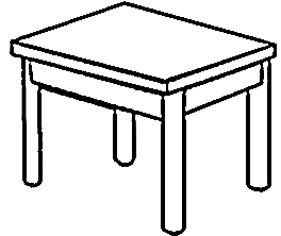
\includegraphics[scale=0.6]{image/mesa.jpg}
\caption{Ejemplo de mesa a fotografía.}
\label{fig:mesa}
\end{figure}

Por lo tanto, se usará PCA con a los 8 indicadores económicos se procede a calcular el nuevo ´índice de marginación. El cuál sería proyectar nuestros indicadores en el primer componente, por definición este tendrá la mayor proporción de la información (varianza) de los datos. Cabe mencionar el PCA no es robusto a escalas, lo que se recomienda en la mayoría de los casos normalizar antes.

\subsection{Replicación del Índice.}
En esta sección replicamos la metodología explicada en la sección anterior de CONAPO pero solo al estado de Nuevo León. \textbf{Hacer este pequeño cambio cambiara un poco los índices, debido a que se estaría perdiendo información de la relación de los índices fuera del estado de Nuevo León. Cabe mencionar que el archivo que se nos paso del Censo 2010 (censo$_$nl.csv) esta desactualizado con la versión  del índice calculado de CONAPO,} esta afirmación se basa a que para crear el índice 2 (de la lista anterior) se necesitaban ciertas columnas que no estaban en el archivo ni en el diccionario de datos. Para arreglar esto y poder replicar completamente la metodología de CONAPO se descargo el archivo del Censo 2010 más actualizado. Con este ajuste la diferencia en los cálculos ahora son mínimos o nulos \cite{conapo}. \\

Nuevo León cuenta con un total de 5262 localidades registradas de las cuales 3224 no tiene ningún registro para calcular los índices. Estas localidades tiene su información confidencial por lo que no podemos realizar un método de imputación ya que estarías sesgando al indicador por que representan más del $50\%$ de las localidades, pero estas 3224 localidades no representan ni el $1\%$ de la población total por lo que podemos ignorarlas para el calculo (esto mismo se hace en el documento de CONAPO). Entonces, el calculo de los índices socioeconómicos se realizo a 2037 localidades, de las cuales solo 1 tenía un valor nulo por lo que se procedió a imputar con la media del municipio considerando el peso que representa la localidad. \\

Antes de aplicar PCA a nuestro conjunto de datos $(2037\times 8)$ los estandarizamos, es decir, a cada observación le restamos la media y esto lo dividimos entre su desviación estándar. Observando la figura \ref{fig:correlaltion} podemos observar que \textbf{la correlación más alta se dan entre el índice de viviendas sin energía eléctrica y viviendas que no disponen de refrigerador con 0.72}, lo cual tiene sentido debido a que si no se cuenta con energía eléctrica esto implica que no tenga un refrigerado ya que no funcionara. 
\begin{figure}[H]
    \centering
    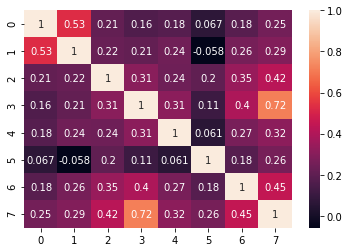
\includegraphics[scale=0.7]{image/correlation.png}
    \caption{Matriz de correlación de los índices socieconomicos.}
    \label{fig:correlaltion}
\end{figure}
La varianza explicada por el primer componente principal es de $37.14\%$ (ver Cuadro \ref{tab:var_explicada}) que a diferencia del reportado por CONAPO hay una diferencia de 9 puntos abajo, esto se explica por el hecho de que no se considera los demás estados. 
\begin{table}[H]
    \centering
    \begin{tabular}{cccc}
        Componentes principales& $\lambda_i$ & Varianza explicada & Varianza acumulada  \\ \hline \hline
        1 & 2.97 & 37.14 &37.14\\
        2 & 1.28 & 15.93 &53.07\\
        3 & 0.25 & 11.84 &64.91\\
        4 & 0.44 &  9.63 &74.54\\
        5 & 0.95 &  8.83 &83.37\\
        6 & 0.64 &  8.03 &91.4\\ 
        7 & 0.71 &  5.47 &96.87\\
        6 & 0.77 &  3.13 &100\\ \hline \hline 
    \end{tabular}
    \caption{Valores propios de la matriz de correlaciones y porcentaje de varianza explicada, 2010}
    \label{tab:var_explicada}
\end{table}
Entonces ocupemos los valores del primer componente principal (ver Cuadro \ref{tab:cp_1}) para calcular el índice de marginación por localidad, para ello solo basta con multiplicar para cada localidad los coeficientes encontrados por los índices socioeconomicos.   
\begin{table}[H]
    \centering
    \begin{tabular}{lc}
        Indicador socioeconómico & coeficientes\\ \hline \hline
        Porcentaje de población de 15 años o más analfabeta. & 0.291 \\
        Porcentaje de población de 15 años o más sin primaria completa. & 0.321\\
        Porcentaje de ocupantes en viviendas particulares habitadas sin drenaje ni excusado. & 0.36\\
        Porcentaje de ocupantes en viviendas habitadas particulares habitadas sin energía eléctrica. & 0.425 \\
        Porcentaje de ocupantes en viviendas particulares habitadas sin agua entubada. & 0.312\\
        Porcentaje viviendas particulares habitadas con algún nivel de hacinamiento. &  0.17  \\
        Porcentaje de ocupantes en viviendas particulares habitadas con piso de tierra. & 0.385\\
        Porcentaje de viviendas particulares habitadas que no disponen de refrigerador. & 0.478\\ \hline \hline 
    \end{tabular}
    \caption{Coeficientes de la primera componente principal por indicador socioeconómicos, 2010}
    \label{tab:cp_1}
\end{table}
Una vez calculado el valor del índice para las 2037 localidades, se procedió a clasificarlas en uno de los cinco grupos proporcionados por CONAPO (ver el Cuadro \ref{tab:limites_marginacion}). Usando estos límites por grupo tenemos la distribución de las localidades que se ve en la Figura \ref{fig:conteo_grupos}. 

\begin{table}[H]
    \centering
    \begin{tabular}{cc}
        Grado de marginación & Límites del IM \\ \hline \hline
        Muy bajo & $[-1.83197, \ \ -1.32309]$\\
        Bajo & $(-1.32309, \ \  -1.06870]$\\
        Medio & $(-1.06870, \ \ -0.81425]$\\
        Alto & $(-0.81425, \ \ 0.71231]$\\
        Muy alto& $(0.71231, \ \ 8.34515]$\\ \hline \hline
    \end{tabular}
    \caption{Clasificación del grado de marginación.}
    \label{tab:limites_marginacion}
\end{table}
El ejemplo más emblemático es el de Nuevo León, aunque se ubica entre las entidades con muy bajo grado de marginación, por localidad se observa que de sus 2 037 localidades, 124 reportan un grado de marginación muy alto $(6.1\%)$, 1030 tienen grado alto $(50.6\%)$, 404 están con grado medio $(19.8\%)$, 321 en grado de marginación bajo $(15.8\%)$ y 158 tienen grado de marginación muy bajo $(7.8\%)$. Esta distribución de las localidades por grado de marginación se parecen bastante a los reportados por CONAPO usando su índice, por lo que podemos concluir que nuestro índice es muy cercano al que reporta CONAPO para Nuevo León.
\begin{figure}[H]
    \centering
    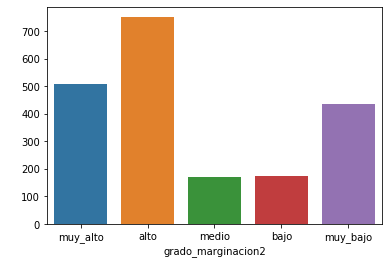
\includegraphics{image/conteo_grupos.png}
    \caption{Localidades por nivel de marginación}
    \label{fig:conteo_grupos}
\end{figure}
Y por último, \textbf{algo importante que resaltar es que la localidad de San Pedro Garza García se encuentra con un índice de marginación muy bajo, están en el top 20 menos marginados lo que hace pensar que el índice es bueno}. Aunque creo que se hubiera esperado que esta localidad estuviera en el top 5 ya que es una de las localidades más importantes.

\subsection{Propuesta para un nuevo índice.}
Los dos planteamientos planteo para mejorar el índice de CONAPO sería: \textbf{ampliar las variables del ámbito individual y integrar aspectos generales.} Con el primer planteamiento me refiero a que las aspectos que considero el CONAPO no es el adecuado o faltan profundizar más. Por ejemplo, el indicador \textit{proxy} sobre el ingreso fue considerando si las viviendas tenían refrigerador, pero observamos que esta variable estaba muy relacionado con si la vivienda contaba electricidad y por lo que pienso que no es un buen estimador del ingreso. Entonces yo sugeriría considerar como el porcentaje de personas que se dedican al sector primario, secundario y terciario, o incluso considerar si la vivienda cuenta con internet o uso del automóvil sería un mejor estimador del ingreso pero tengo entendido que en el Censo 2010 no se tenía esa información. \\  

Por otro lado, el segundo planteamiento me refiero a considerar aspectos generales de las localidades y así complementar el índice propuesto. \textbf{Con aspectos más generales me refiero por ejemplo así en la localidad existen bancos, hospitales, escuelas, centros comerciales, ¿cuántos existen? Y si no hay en la localidad, entonces cuál es la distancia a la localidad más cerca que los tenga.} De cierta manera considerar estos aspectos dan un enfoque general de la población en general, porque contar con los servicios más utilizados (salud, finanzas, etc) en los últimos años esta relacionado con el grado de marginalidad de cada localidad. \\

Una manera de poder crear este índice sería considerando el Directorio Estadístico Nacional de Unidades Económicas (DENUE) el cual realiza el INEGI. Este directorio cuenta con cada unidad económica del país, de donde podríamos calcular el número el número de hospitales, escuelas, bancos, centros comerciales o la distancia más cerca a estos lugares por localidad. Y con esto podrías realizar un nuevo índice para complementar a los  anteriores.  \textbf{Otro aspecto general que se puede considerar sería la delincuencia}, este índice se esperaría que en los lugares más marginales y con los niveles más marginales tengan un índice que delincuencia menor en cambio los lugares con niveles moderados de marginación tendrían un mayor más grande. Este índice se puede construir con los reportes diarios de delitos estatales. Y por último, \textbf{podríamos considerar el porcentaje de calles que se encuentran pavimentadas o rusticas}, esto nos daría un enfoque de esta la construcción de las localidades lo cual estaría muy relacionado debido a que es más difícil pavimentar en lugares con más marginación es más difícil y caro llevar el material, trabajadores y maquinaria que en lugares menos marginales.  \\

Un problema por el cuaĺ no se calcularon el nuevo índice propuesto fue debido a que actualmente no se encuentra las limitaciones de las localidades de México, es decir, no se tienen geodelimitadas las localidades. Esto hace imposible calcular por ejemplo el número de hospitales en cada localidad, ya que no sabríamos saber a que localidad le pertenece. 
\subsection{Conclusiones.}
En general podría decir que el índice que propone CONAPO es adecuado para clasificar el grado de marginación. Pero algo importante a notar es que no es están bueno para aspectos más específicos. Como el presupuesto de cada municipio depende de este índice creo que debería comprender más aspectos para que este mejor. Lo anterior se debe a la clasificación de la localidad de San Pedro Garza García ya que no se encuentra en un nivel más bajo. \\

Por otro lado, creo que este índice no es tan informativo. Ya que no podríamos saber que factor es que tendría que mejorar para tener una mayor clasificación. Por lo que si estamos interesados en políticas públicas para disminuir el grado de marginación en las localidades sería complicado buscar propuestas para hacerlo.

\section{Eigenfaces}
En este ejercicio nos enfocamos al conjunto de datos Labelled Faces in the Wild, que consiste en fotografías de rostros recolectados de internet y contenido en \texttt{sklearn}. Solo se consideraron aquellas personas que tienen al menos 70 fotografías de su rostro en su tamaño original de la imagen $(125 \times 94)$. 

\subsection{a) Primeros dos componentes.}
El número total de imágenes analizadas fueron 1288, algo importante a resaltar es la proporción de fotografías que se encuentra en la muestra por cada personaje. Observamos que existe una muestra desbalanceada lo que puede influir en los errores, dándoles más prioridad a George W Bush por ser el que tiene más imágenes a la muestra (Ver Cuadro \ref{tab:conteo_imagenes}).

\begin{table}[H]
    \centering
    \begin{tabular}{c|c}
         Nombre& Número de Fotografia \\ \hline \hline
         George W Bush  &  530\\
Colin Powell    & 236\\
Tony Blair      & 144\\
Donald Rumsfeld & 121\\
Gerhard Schroeder  & 109\\
Ariel Sharon    &77\\
Hugo Chavez     &71\\ \hline \hline
    \end{tabular}
    \caption{Número de fotografías por personaje en la muestra.}
    \label{tab:conteo_imagenes}
\end{table}

Se realizó una partición de nuestros datos en un conjunto de entrenamiento ($\%80$) y conjunto de prueba. Posteriormente llevamos acabo la metodología de PCA para encontrar los eigenfaces en nuestros conjunto de entrenamiento. Observando los dos primeros componentes principales podemos dar una "explicación de estos", el primer componente principal se enfoca en los rasgos del rostro: los ojos, nariz y boca. Y el segundo componente principal se enfoca en el fondo de la imagen.
\begin{figure}[H]
    \centering
    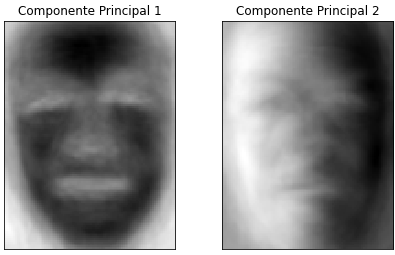
\includegraphics[scale=0.8]{image/two_pc.png}
    \caption{Primeros 2 componentes principales.}
    \label{fig:two_pc}
\end{figure}
Por otro lado, la varianza explicada por estos dos componentes es aproximadamente $38\%,$ es un valor muy bajo por lo que se sugeriría usar un número mayor de componentes principales para tener mejores resultados en cualquier análisis. 

\subsection{Ubicación de cada individuo.}
Ahora consideremos las proyecciones de los datos en los primeros dos componentes principales encontrados. \\

Al graficarlos en el plano cartesiano no podemos tener una segmentación de los datos, es decir, se esperaría que podamos separar las proyecciones de los datos en 8 grupos diferentes y cada grupo significará una persona (Ver Figura \ref{fig:graph_two_cp}). \\

Las dos razones que puedo dar por la cual no se observa lo esperado son: la primera se puede deber a que como los dos componentes principales utilizados no explican un porcentaje alto de la varianza esto hace que no se este recopilando mucha información de los datos para obtener una segmentación por cada personaje. Y la segunda es debido a que no exista una segmentación como nosotros la vemos, es decir, en lugar de separar por persona los componentes principales estén segmentando por características del rostro: ojos grandes, nariz corpulenta, uso de anteojos, etc.
\begin{figure}[H]
    \centering
    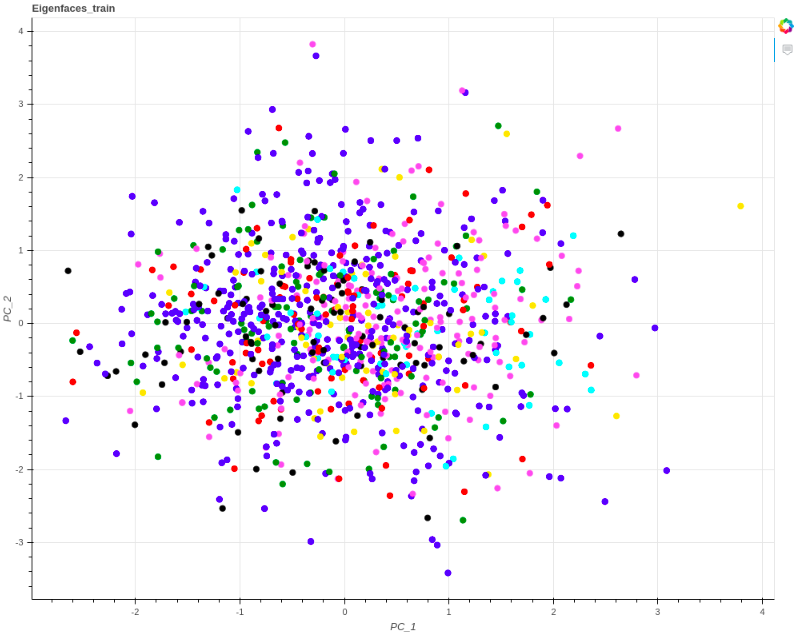
\includegraphics[scale=0.6]{image/graph_two_cp.png}
    \caption{Proyecciones de los datos en los 2 primeros componentes principales.}
    \label{fig:graph_two_cp}
\end{figure}
Ahora proyectemos los datos de prueba en la figura \ref{fig:graph_two_cp} y veamos algunos ejemplos de qué fotografía es el más cercana. En la figura \ref{fig:proyeccion} se pueden observar la fotografía 125 y 15 de los datos de entrenamiento, cada una se proyecta en los primeros dos componentes y se encuentra la fotografía más cerca (considerando la distancia euclidiana) de los primeros dos componentes. La primera imagen que muestra a Gerhard Schoreder podemos ver que la imagen más cerca no es de el sino de Colin Powell, en cambio la segunda imagen de George W Bush observamos que la imagen más cerca si le pertenece a el.  
\begin{figure}[H]
    \centering
    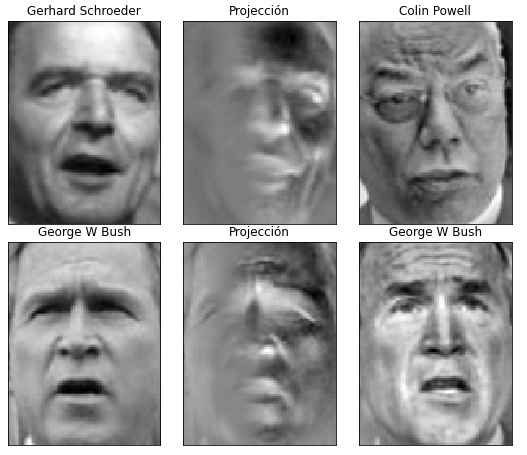
\includegraphics[scale=0.6]{image/proyeccion.png}
    \caption{Proyección de los datos de prueba en dos componentes principales.}
    \label{fig:proyeccion}
\end{figure}
Si buscamos la imagen más cerca a cada una de las proyecciones de las imagenes de prueba tendríamos que $24.8\%$ de las proyecciones estaría cerca a una imagen con el personaje que le corresponde, \texbf{lo que implica que en el $75\%$ de las veces no estaría ubicando bien a los individuos.} 

\subsection{Identificación de la persona en la imagen.}
El objetivo de esta sección es poner clasificar las imágenes según el personaje que aparece en estas. Para ello ocupamos la metodología del vecino más cercano, utilizando la distancia euclidiana como medida de disimilaridad. En la sección anterior se puede interpretar como el vecino más cercano considerando solo dos componentes principales, y ya vimos que no generan buenos resultados con pocos componentes. \\

Tengamos en cuenta que el número de componentes principales a ocupar en las proyecciones y el número de vecinos más cercano son parámetros que afectan en el  los errores de clasificación. Estos parámetros son muy influyentes en la clasificación de las imágenes, por lo que es importante saber que combinación de parámetros elegir. \\

Para ello, un enfoque para saber la cantidad de componentes principales a ocupar es tomando en cuenta la varianza acumulada por los componentes principales. Si consideramos los primeros 50 componentes principales tenemos aproximadamente $80\%$ de la varianza de los datos explicada, si consideramos los primeros 100 componentes principales tenemos aproximadamente $90\%$ de la varianza. Entonces si consideramos $50$ ya sería "sucifiente" para tener un buen predictor. 
\begin{figure}[H]
    \centering
    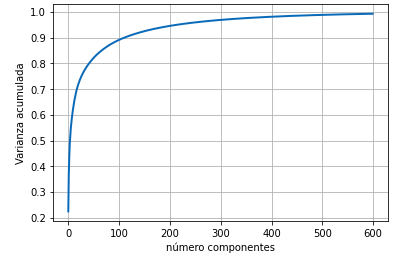
\includegraphics[scale=0.6]{image/var_acumulad.png}
    \caption{Varianza acumulada explicada por los componentes principales.}
    \label{fig:var_acumulad}
\end{figure}
La segunda manera de abordar la incertidumbre que proporcionan los parámetros es considerar es considerar diversas combinaciones de parámetros y considerar la combinación con el error más pequeño, utilizando validación cruzada. Esta metodologías conocida como Hyperparameter tuning methods se enfocan básicamente en configurar de antemano los hiperparámetro de los algoritmos de aprendizaje automático para obtener un rendimiento predictivo óptimo mediante un procedimiento de ajuste. \cite{tunability} Entonces, \textbf{ocupando lo anterior con la ayuda de la librería sklearn pudimos encontrar que ocupando $p=60$ y $n\_neighbors=6$ es la combinación de parámetros con el menor error de todas las combinaciones que se probaron, el error utilizando validación cruzada fue de 0.703 (sin utilizar validación cruzada fue de 0.846)}.\\

\begin{lstlisting}[style=customc,basicstyle=\scriptsize]
    from sklearn.pipeline import Pipeline
    from sklearn.model_selection import GridSearchCV

    pca = PCA(svd_solver='randomized', whiten=True).fit(X_train)
    knn = KNeighborsClassifier(p=2)

    pipe = Pipeline(steps=[('pca', pca), ('knn', knn)])

    param_grid = {
    'pca__n_components': [5, 15, 45, 60, 90, 120, 135, 150, 120],
    'knn__n_neighbors': [1, 3, 6, 9, 10, 12, 13]
    }

    search = GridSearchCV(pipe, param_grid, n_jobs=-1)
    search.fit(X_train, y_train)
\end{lstlisting}  
Ahora, considerando la combinación anterior \textbf{el error obtenido en el conjunto de prueba fue de 0.732. Por lo que podemos concluir que el ajuste del modelo es adecuado.} En la Figura \ref{fig:neighbors} podemos observar la imagen sin modificaciones, normalizada, las proyecciones en los 60 componentes principales y el vecino más cercano con la probabilidad de ser clasificado con ese personaje. Es decir, en la primeras imágenes observamos al ex-presidente George W. Bush el cual el algoritmo del vecino más cercano lo clasificó como George W. Bush con una probabilidad de 1. En las imágenes posteriores observamos al ex-presidente alemán Gerhard Schroeder el cuál el cual el algoritmo del vecino más cercano lo clasificó como Gerhard Schroeder con una probabilidad de 0.5, es decir, de los otros 7 personajes tiene el resto de la probabilidad. 
\begin{figure}[H]
    \centering
    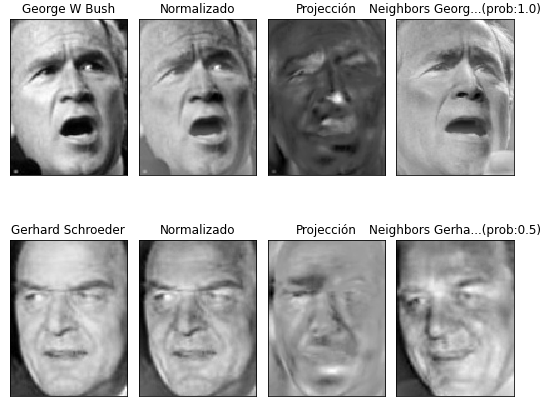
\includegraphics[scale=0.6]{image/neighbors.png}
    \caption{Identificación utilizando KNN.}
    \label{fig:neighbors}
\end{figure}
\subsection{Prevención de casos.}
Una manera de disminuir el error o posibles errores de clasificación es considerar un umbral más estricto en el algoritmo del vecino más cercano. Nosotros podemos obtener la probabilidad de cada personaje cuando se quiere clasificar una imagen, entonces si observamos que la probabilidad máxima de todos los personajes es menor a $50\%$ entonces podríamos clasificar la nueva imagen como: imposible clasificar.\\
En la figura \ref{fig:vicente_fox} podemos observar la imagen del ex presidente de México Vicente Fox, el cual si lo proyectamos en los 60 componentes principales y usamos buscamos los vecinos más cercanos, tendríamos que la probabilidad más alta la tiene Colin Powell por lo que con nuestra regla de decisión a esta nueva imagen la clasificaríamos como: imposible de clasificar. 
\begin{figure}[H]
    \centering
    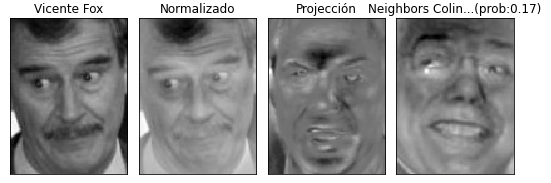
\includegraphics[scale=0.6]{image/vicente_fox.png}
    \caption{Vicente Fox clasificación: imposible de clasificar.}
    \label{fig:vicente_fox}
\end{figure}
Otro enfoque sería considerar las distribución de la distancias de los 6 vecinos más cercanos. Y si la distancia de la nueva a sus 6 vecinos más cercanos no cae en los 2 y 3 cuantiles podríamos considerar que esa foto no es de alguien de la muestra. Pero este enfoque es equivalente a obtener las probabilidades que proporciona el algoritmo de vecino más cercanos programado en \texttt{sklearn.}

\section{Problema 4}
Dado un conjunto de datos centrados $X_{n\times d}$, vimos que hacer PCA, es realizar la descomposición espectral de la matriz de covarianzas muestral, que puede estimarse como $S=X'X$ (omitimos el coeficiente $n-1$). Ahora, considera la matriz $K_{n\times n}= \bf{XX}'.$

\subsection{Realizar PCA utilizando la matriz $\bf S$ es equivalente a hacerlo en con la matriz $\bf K$}
Recordemos la definición de valor propio y vector propio de una matriz.

\begin{framed}
    \begin{thmd} \label{d_eigenvalor}
	Sea $A$ una matriz de $n\times n$. El escalar $\lambda$ es un valor propio de $A$ si el vector $x (x\neq 0)$ se cumple
	$$A\bf x =\lambda x.$$
	El vector $x$ es el vector propio de $A$ correspondiente a $\lambda.$ \cite{algebra_lineal_1}
    \end{thmd}
\end{framed}

Ocupando la Definición \ref{d_eigenvalor}, sea $\lambda$ un valor propio de la matriz $\bf S$ y $\bf u$ su vector propio correspondiente, entonces 
\begin{align*}
    \bf Su &= \bf \lambda u\\
    \bf X'X u   &= \bf \lambda u\\
    \bf X X'X u &= \bf X\lambda u\\
    \bf X X' (Xu)&=\bf \lambda (Xu)\\
    \bf K (Xu) &= \bf \lambda (Xu).
\end{align*}
Por lo anterior, podemos concluir que $\lambda$ también es valor propio de la matriz $K$ con vector propio correspondiente $Xu$. También veamos que,
\begin{align*}
    \bf Su &= \bf \lambda u\\
    \bf X'X u   &= \bf \lambda u\\
    \bf u^TX'X u &= \bf u^T\lambda u\\
    \bf || Xu||^2 & = \bf \lambda u^T u = \lambda. \Rightarrow ||Xu|| =\sqrt{\lambda}.
\end{align*}
Entonces podemos concluir que el vector propio de $\lambda$ normalizado para la matriz $K$ es $\frac{Xu}{||Xu||}=\lambda^{-1/2}Xu.$ Y de igual manera, sea $\lambda$ valor propio de $K$ y $\bf{v}$ su vector propio correspondiente, entonces
\begin{align*}
    \bf Kv &= \bf \lambda v\\
    \bf XX' v   &= \bf \lambda v\\
    \bf X' XX' v &= \bf X'\lambda v\\
    \bf X' X (X'v)&=\bf \lambda (X'v)\\
    \bf S (X'v) &= \bf \lambda (X'v).
\end{align*}
Entonces, podemos concluir que $\lambda$ también es valor propio de la matriz $S$ con vector propio correspondiente $X'v$. También veamos que,
\begin{align*}
    \bf Kv &= \bf \lambda u\\
    \bf XX' v   &= \bf \lambda v\\
    \bf v^TXX' v &= \bf v^T\lambda v\\
    \bf || X'v||^2 & = \bf \lambda v^T v = \lambda. \Rightarrow ||X'v|| =\sqrt{\lambda}.
\end{align*}
Entonces podemos decir que el vector propio de $\lambda$ normalizado para la matriz $S$ es $\frac{X'v}{||X'v||}=\lambda^{-1/2}'X'v.$ \textbf{Por lo tanto, se ha demostrado que $(\lambda^{-1/2})Xu, \lambda$ es un par de vector propio normalizado y valor propio de la matriz $\bf K$, y a su vez, $(\lambda^{-1/2})X^Tv, \lambda)$ es un par de vector propio normalizado y valor propio de la matriz $\bf S$, donde $\bf u$ y $\bf v$ son vectores propios de $\bf S$ y $\bf K$ respectivamente. Y lo anterior implica que realizar PCA en $\bf S$ es equivalente a realizarlo ocupando la matriz $\bf K$.}


\subsection{Ejemplo de PCA con la matriz $\bf K$.}
Para observar que hacer PCA en la matriz $\bf K$ es equivalente a hacerlo en la matriz $\bf S$, procedemos a  obtener los valores propios de ambas matrices y compararemos los primeros 5 componentes principales en el conjunto de datos de las imágenes LFW de la sección anterior. Realizando esto ocupando la librería \texttt{sklearn} obtenemos los eigenfaces que se observan en la figura \ref{fig:eigenfaces_matrix}. En ella podemos observar los primeros eigenfaces obtenidos con la matriz $\bf S$ en la parte de arriba y en la parte de abajo los eigenfaces obtenidos con la matriz $\bf K$. Lo cual podemos observar claramente que son los mismos. Al tomar el tiempo de ejecución vimos un tiempo más pequeño cuando se ocupo la matriz $\bf K$.
\begin{figure}[H]
    \centering
    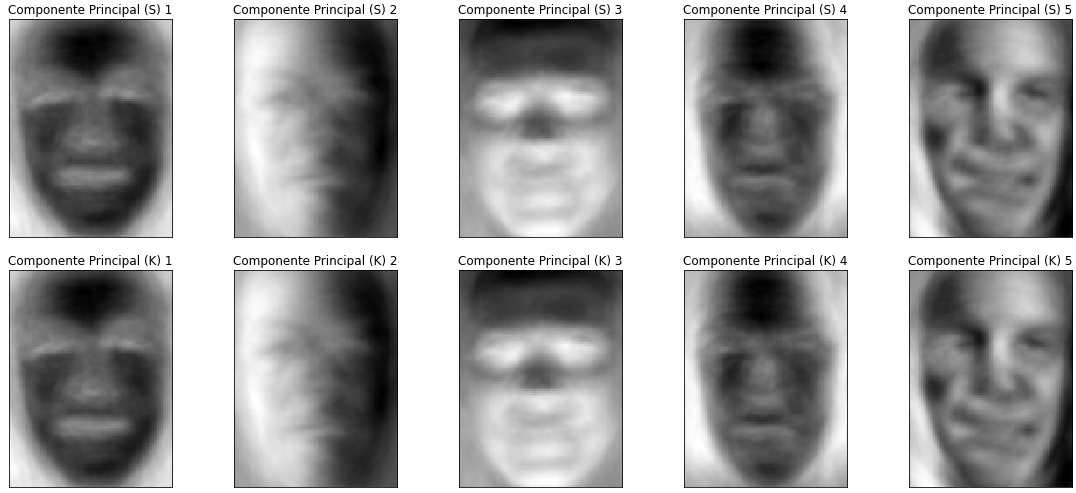
\includegraphics[scale=0.4]{image/eigenfaces_matrix.png}
    \caption{Eigenfaces usando la matriz $\bf S$ y $\bf K$ respectivamente.}
    \label{fig:eigenfaces_matrix}
\end{figure}

En el caso cuando el número de registros $n$ es más grande que el número de variables del conjunto de datos, es mejor recomendable trabajar con la matriz $\bf S$, ya que tendrá dimensiones más pequeñas que la matriz $\bf K$. Ahora, en el caso que el número de registros sea menor que el número de variables (esto es muy común en áreas como la genética) entonces es recomendable utilizar la matrizz $\bf K$ ya que será de un tamaño más pequeño y esto facilitaría los cálculos para encontrar los valores y vectores propios. Esto es lo que paso en este ejemplo, en donde el número de registros era mucho más pequeño que las variables del conjunto de datos, ya que el tiempo de ejecución fue menor cuando se utilizó la matriz $\bf K$ para encontrar los eigenfaces.   
\section{Anexos.}
\subsection{Códigos.}
Todos los códigos utilizados para estos resultados se pueden encontrar en mi página personal de Gitgub: Enriquesec. En el repositorio \texit{ Ciencia$\_$de$\_$Datos/Tareas/Tareas$_$2/solution.ipynb}

\subsection{Calculos de los Indicadores socioeconómicos.}
Cómo ya se menciono en la sección 2.3 el conjunto de datos que se nos proporciono estaba desactualizado, por lo que se descargo de la página \texit{https://www.inegi.org.mx/programas/ccpv/2010/?ps=microdatos}. Para calcular los 8 índices socioeconomicos se ocuparon las siguientes columnas y formulas:\\

\begin{itemize}
    \item Porcentaje de población de 15 años o más analfabeta. 
    \begin{itemize}
        \item  Población de 15 años o más $\left(P_i^{15+}\right)$. Columna: $\bf P\_15YMAS$.
        \item Población de 15 años o más analfabeta $\left(P_i^{anal}\right)$: Columna: $\bf P15YM_AN$.
    \end{itemize}
    $$\text{Calculo del índice }I_{i,1}=\frac{P_i^{anal}}{P_i^{15+}}*100.$$
    
    \item Porcentaje de población de 15 años o más sin primaria completa.
    \begin{itemize}
        \item Población de 15 años o más sin escolaridad $\left(P_i^{15+se}\right)$. Columna: $\bf P15YM\_SE$. 
        \item Población de 15 años o más con primaria incompleta $\left(P_i^{15+pin}\right)$. Columna: $\bf P15PRI\_IN$.
        \item Población de 15 años o más con primaria completa $\left(P_i^{15+pco}\right)$. Columna: $\bf P15PRI\_CO$.
        \item Población de 15 años o más con secundaria incompleta $\left(P_i^{15+sse}\right)$. Columna: $\bf P15SEC\_IN$.
        \item Población de 15 años o más con secundaria completa $\left(P_i^{15+sco}\right)$. Columna: $\bf P15SEC\_CO$.
        \item Población de 18 años o más con educación pos-básica $\left(P_i^{18+pb}\right)$. Columna: $\bf P18YM\_PB$.
    $$\text{Calculo del índice } I_{i,2}=\frac{P_i^{15+se}+P_i^{15+pin}}{P_i^{15+se}+P_i^{15+pin}+P_i^{15+pco}+P_i^{15+sse}+P_i^{15+sco}+P_i^{15+pb}}$$
    \end{itemize}
    \item Porcentaje de viviendas particulares habitadas sin excusado.
    \begin{itemize}
        \item Total de viviendas particulares habitadas$\left(P_i^{tvv}\right)$. Columna: $\bf TVIVPARHAB$.
        \item Total viviendas particulares habitadas que disponen de excusado o sanitario$\left(P_i^{tvv\_exc}\right)$. Columna: $\bf VPH\_EXCSA$.
        $$\text{Calculo del índice } I_{i,3}=\frac{P_i^{tvv}-P_i^{tvv\_exc}}{P_i^{tvv}}.$$
    \end{itemize}
    \item Porcentaje de viviendas particulares habitadas sin energía eléctrica.
    \begin{itemize}
        \item  Viviendas particulares habitadas que no disponen de luz eléctrica$\left(P_i^{vv\_sl}\right)$. Columna: $\bf VPH\_S\_ELEC$.
        \item Viviendas particulares habitadas que disponen de luz eléctrica$\left(P_i^{vv\_cl}\right)$. Columna $\bf VPH\_C\_ELEC$.
        $$\text{Calculo del índice } I_{i,4}=\frac{P_i^{vv\_sl}}{P_i^{vv\_sl}+P_i^{vv\_cl}}.$$
    \end{itemize}
    \item Porcentaje de viviendas particulares habitadas sin disponibilidad de agua entubada.
    \begin{itemize}
        \item Viviendas particulares habitadas que no disponen de agua entubada en el ámbito de la vivienda$\left(P_i^{vv\_sa}\right)$. Columna: $VPH\_AGUADV$.
        \item Viviendas particulares habitadas que disponen de agua entubada en el ámbito de la vivienda$\left(P_i^{vv\_cl}\right)$. Columna $VPH\_AGUAFV$.
        $$\text{Calculo del índice } I_{i,5}=\frac{P_i^{vv\_sa}}{P_i^{vv\_sa}+P_i^{vv\_ca}}.$$
    \end{itemize}
    
    \item Promedio de ocupantes por cuarto en viviendas particulares habitados (ya calculado) $I_{i,6}$. Columna: $\bf PRO\_OCUP\_C$.
    
    \item Porcentaje de viviendas particulares habitadas con piso de tierra.
    \begin{itemize}
        \item Viviendas particulares habitadas con piso de tierra$\left(P_i^{vv\_ct}\right)$. Columna: $\bf VPH\_PISOTI$.
        \item Viviendas particulares habitadas con piso diferente de tierra$\left(P_i^{vv\_st}\right)$. Columna: $\bf VPH\_PISODT$.
        $$\text{Calculo del índice } I_{i,7}=\frac{P_i^{vv\_ct}}{P_i^{vv\_st}+P_i^{vv\_ct}}.$$
    \end{itemize}
    \item Porcentaje de viviendas particulares habitadas que no disponen de refrigerador.
    \begin{itemize}
        \item Viviendas particulares habitadas totales$\left(P_i^{tvv}\right)$. Columna: $TVIVPARHAB$.
        \item Viviendas particulares habitadas que disponen de refrigerador$\left(P_i^{vv\_cr}\right)$. Columna: $\bf VPH\_REFRI$.
        $$\text{Calculo del índice } I_{i,8}=\frac{P_i^{vv\_cr}}{P_i^{tvv}}.$$
    \end{itemize}
\end{itemize} 
Con lo anterior sería suficiente de calcular de los índices de las localidades de Nuevo León sin ningún problema. 
\printbibliography

\end{document}
